\documentclass{standalone}
\usepackage{tikz}
\usepackage{ctex,siunitx}
\usepackage{tkz-euclide}
\usepackage{amsmath}
\usetikzlibrary{patterns, calc}
\usetikzlibrary {decorations.pathmorphing, decorations.pathreplacing, decorations.shapes,}
\begin{document}
\small
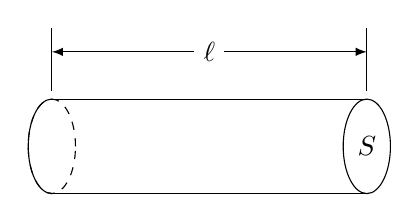
\begin{tikzpicture}[>=latex,scale=1.0]
  \draw(0,.6)--(4,.6);
  \draw(0,-.6)--(4,-.6);
  \draw[dashed](0,0)ellipse[x radius=.3, y radius=.6]; 
  \draw (4,0)node[]{$S$} ellipse[x radius=.3, y radius=.6]; 
  \draw(0,.7)--(0,1.5);
  \draw(4,.7)--(4,1.5);
  \draw[<->](4,1.2)--node[fill=white]{$\ell$}(0,1.2);
  \draw(0,.6) arc [start angle = 90, end angle=270, x radius=.3, y radius=.6];
\end{tikzpicture}
\end{document}